% Options for packages loaded elsewhere
\PassOptionsToPackage{unicode}{hyperref}
\PassOptionsToPackage{hyphens}{url}
\PassOptionsToPackage{dvipsnames,svgnames,x11names}{xcolor}
%
\documentclass[
  a4paper,
  DIV=11,
  numbers=noendperiod]{scrartcl}

\usepackage{amsmath,amssymb}
\usepackage{iftex}
\ifPDFTeX
  \usepackage[T1]{fontenc}
  \usepackage[utf8]{inputenc}
  \usepackage{textcomp} % provide euro and other symbols
\else % if luatex or xetex
  \usepackage{unicode-math}
  \defaultfontfeatures{Scale=MatchLowercase}
  \defaultfontfeatures[\rmfamily]{Ligatures=TeX,Scale=1}
\fi
\usepackage{lmodern}
\ifPDFTeX\else  
    % xetex/luatex font selection
\fi
% Use upquote if available, for straight quotes in verbatim environments
\IfFileExists{upquote.sty}{\usepackage{upquote}}{}
\IfFileExists{microtype.sty}{% use microtype if available
  \usepackage[]{microtype}
  \UseMicrotypeSet[protrusion]{basicmath} % disable protrusion for tt fonts
}{}
\makeatletter
\@ifundefined{KOMAClassName}{% if non-KOMA class
  \IfFileExists{parskip.sty}{%
    \usepackage{parskip}
  }{% else
    \setlength{\parindent}{0pt}
    \setlength{\parskip}{6pt plus 2pt minus 1pt}}
}{% if KOMA class
  \KOMAoptions{parskip=half}}
\makeatother
\usepackage{xcolor}
\usepackage[top=25mm,left=40mm,right=30mm,bottom=25mm,heightrounded]{geometry}
\setlength{\emergencystretch}{3em} % prevent overfull lines
\setcounter{secnumdepth}{-\maxdimen} % remove section numbering
% Make \paragraph and \subparagraph free-standing
\makeatletter
\ifx\paragraph\undefined\else
  \let\oldparagraph\paragraph
  \renewcommand{\paragraph}{
    \@ifstar
      \xxxParagraphStar
      \xxxParagraphNoStar
  }
  \newcommand{\xxxParagraphStar}[1]{\oldparagraph*{#1}\mbox{}}
  \newcommand{\xxxParagraphNoStar}[1]{\oldparagraph{#1}\mbox{}}
\fi
\ifx\subparagraph\undefined\else
  \let\oldsubparagraph\subparagraph
  \renewcommand{\subparagraph}{
    \@ifstar
      \xxxSubParagraphStar
      \xxxSubParagraphNoStar
  }
  \newcommand{\xxxSubParagraphStar}[1]{\oldsubparagraph*{#1}\mbox{}}
  \newcommand{\xxxSubParagraphNoStar}[1]{\oldsubparagraph{#1}\mbox{}}
\fi
\makeatother


\providecommand{\tightlist}{%
  \setlength{\itemsep}{0pt}\setlength{\parskip}{0pt}}\usepackage{longtable,booktabs,array}
\usepackage{calc} % for calculating minipage widths
% Correct order of tables after \paragraph or \subparagraph
\usepackage{etoolbox}
\makeatletter
\patchcmd\longtable{\par}{\if@noskipsec\mbox{}\fi\par}{}{}
\makeatother
% Allow footnotes in longtable head/foot
\IfFileExists{footnotehyper.sty}{\usepackage{footnotehyper}}{\usepackage{footnote}}
\makesavenoteenv{longtable}
\usepackage{graphicx}
\makeatletter
\newsavebox\pandoc@box
\newcommand*\pandocbounded[1]{% scales image to fit in text height/width
  \sbox\pandoc@box{#1}%
  \Gscale@div\@tempa{\textheight}{\dimexpr\ht\pandoc@box+\dp\pandoc@box\relax}%
  \Gscale@div\@tempb{\linewidth}{\wd\pandoc@box}%
  \ifdim\@tempb\p@<\@tempa\p@\let\@tempa\@tempb\fi% select the smaller of both
  \ifdim\@tempa\p@<\p@\scalebox{\@tempa}{\usebox\pandoc@box}%
  \else\usebox{\pandoc@box}%
  \fi%
}
% Set default figure placement to htbp
\def\fps@figure{htbp}
\makeatother
% definitions for citeproc citations
\NewDocumentCommand\citeproctext{}{}
\NewDocumentCommand\citeproc{mm}{%
  \begingroup\def\citeproctext{#2}\cite{#1}\endgroup}
\makeatletter
 % allow citations to break across lines
 \let\@cite@ofmt\@firstofone
 % avoid brackets around text for \cite:
 \def\@biblabel#1{}
 \def\@cite#1#2{{#1\if@tempswa , #2\fi}}
\makeatother
\newlength{\cslhangindent}
\setlength{\cslhangindent}{1.5em}
\newlength{\csllabelwidth}
\setlength{\csllabelwidth}{3em}
\newenvironment{CSLReferences}[2] % #1 hanging-indent, #2 entry-spacing
 {\begin{list}{}{%
  \setlength{\itemindent}{0pt}
  \setlength{\leftmargin}{0pt}
  \setlength{\parsep}{0pt}
  % turn on hanging indent if param 1 is 1
  \ifodd #1
   \setlength{\leftmargin}{\cslhangindent}
   \setlength{\itemindent}{-1\cslhangindent}
  \fi
  % set entry spacing
  \setlength{\itemsep}{#2\baselineskip}}}
 {\end{list}}
\usepackage{calc}
\newcommand{\CSLBlock}[1]{\hfill\break\parbox[t]{\linewidth}{\strut\ignorespaces#1\strut}}
\newcommand{\CSLLeftMargin}[1]{\parbox[t]{\csllabelwidth}{\strut#1\strut}}
\newcommand{\CSLRightInline}[1]{\parbox[t]{\linewidth - \csllabelwidth}{\strut#1\strut}}
\newcommand{\CSLIndent}[1]{\hspace{\cslhangindent}#1}

\addtokomafont{disposition}{\rmfamily}
\KOMAoption{captions}{tableheading}
\makeatletter
\@ifpackageloaded{caption}{}{\usepackage{caption}}
\AtBeginDocument{%
\ifdefined\contentsname
  \renewcommand*\contentsname{Table of contents}
\else
  \newcommand\contentsname{Table of contents}
\fi
\ifdefined\listfigurename
  \renewcommand*\listfigurename{List of Figures}
\else
  \newcommand\listfigurename{List of Figures}
\fi
\ifdefined\listtablename
  \renewcommand*\listtablename{List of Tables}
\else
  \newcommand\listtablename{List of Tables}
\fi
\ifdefined\figurename
  \renewcommand*\figurename{Figure}
\else
  \newcommand\figurename{Figure}
\fi
\ifdefined\tablename
  \renewcommand*\tablename{Table}
\else
  \newcommand\tablename{Table}
\fi
}
\@ifpackageloaded{float}{}{\usepackage{float}}
\floatstyle{ruled}
\@ifundefined{c@chapter}{\newfloat{codelisting}{h}{lop}}{\newfloat{codelisting}{h}{lop}[chapter]}
\floatname{codelisting}{Listing}
\newcommand*\listoflistings{\listof{codelisting}{List of Listings}}
\makeatother
\makeatletter
\makeatother
\makeatletter
\@ifpackageloaded{caption}{}{\usepackage{caption}}
\@ifpackageloaded{subcaption}{}{\usepackage{subcaption}}
\makeatother

\usepackage{bookmark}

\IfFileExists{xurl.sty}{\usepackage{xurl}}{} % add URL line breaks if available
\urlstyle{same} % disable monospaced font for URLs
\hypersetup{
  pdftitle={Slap Group Project},
  colorlinks=true,
  linkcolor={blue},
  filecolor={Maroon},
  citecolor={Blue},
  urlcolor={Blue},
  pdfcreator={LaTeX via pandoc}}


\title{Slap Group Project}
\author{}
\date{}

\begin{document}
\maketitle


\subsection*{Declaration of Authorship}\label{declaration-of-authorship}

We, {[}Slap{]}, pledge our honour that the work presented in this
assessment is our own. Where information has been derived from other
sources, we confirm that this has been indicated in the work. Where a
Large Language Model such as ChatGPT has been used we confirm that we
have made its contribution to the final submission clear. Date:
17.12.2024 Student Numbers: 20017452, 24246337, 25000148, 24231390,
24242570. \#\# Brief Group Reflection \textbar{} What Went Well
\textbar{} What Was Challenging \textbar{} \textbar{} --------------
\textbar{} -------------------- \textbar{} \textbar{} A We identified
the project scope early, and spent most of the time on interpretation,
discussion and refinements to EDA \textbar{} B Interpretation of
residuals \textbar{} \textbar{} C We are seeing some impact which we
expected to see \textbar{} D Cleaning and deduplicating the InsideAirbnb
dataset \textbar{} \#\# Priorities for Feedback Are there any areas on
which you would appreciate more detailed feedback if we're able to offer
it? * Our approach to identifying valid airbnbs * Our approach to
interpretation * Our suggestions for future STL regulation

\newpage{}

\section{Response to Questions}\label{response-to-questions}

See the raw file for examples of how to hide computational output as
there is code hidden here.

\subsubsection{Growing number of
listings}\label{growing-number-of-listings}

We identified 28,207 active London listings in 2024 - 55.22\%
year-on-year increase. The listings accounted for 0.48\% and 0.74\% of
total dwellings respectively {`Net additional dwellings'} (2024); entire
homes - 0.35\% and 0.58\% respectively, in contrast to other sources
(Young LLP, 2024). The central areas exhibit the highest proportion of
Airbnb listings relative to total dwellings, and this share increased
progressively across these and adjacent boroughs from 2023 to 2024.
\#\#\# Trend towards entire homes In 2024, the percentage of entire
homes on Airbnb increased to 78\%, up from 73\% in 2023. The share of
private rooms decreased from 26\% to 21\%, indicating a trend towards
more entire homes, which have a greater impact on housing. Some sources
suggest STL ease and higher revenue may incentivize removing properties
from long-term rental markets Andy Evans (2020), even if they start STL
as a private room. We therefore see the need to expand the methodology
to include private rooms into the research scope. \#\#\# More
multi-listing hosts The proportion of multi-listing hosts increased from
53\% in 2023 to 57\% in 2024, with 36\% of these hosts having two
listings. The average number of listings per multi-listing host rose
from 14.8 to 19.5, and nearly 10\% now manage more than 10 listings.
Notably, there is growing prevalence of one-bedroom and 3+ bedroom
listings, suggesting that multi-listing hosts are increasingly occupying
larger homes and one-bedroom properties. This trend may limit access to
family-sized housing and properties for first buyers. The high average
number of listings likely reflects the involvement of asset management
companies, pointing to a trend towards greater commercialisation of the
platform. We compare our observations with the Airbnb-endorsed studies
Kath Scanlon (2024). As seen from our EDA, the commercial use of the
platform is increasing, and the impact on housing could be
underestimated. We discuss it further in the next section.

\pandocbounded{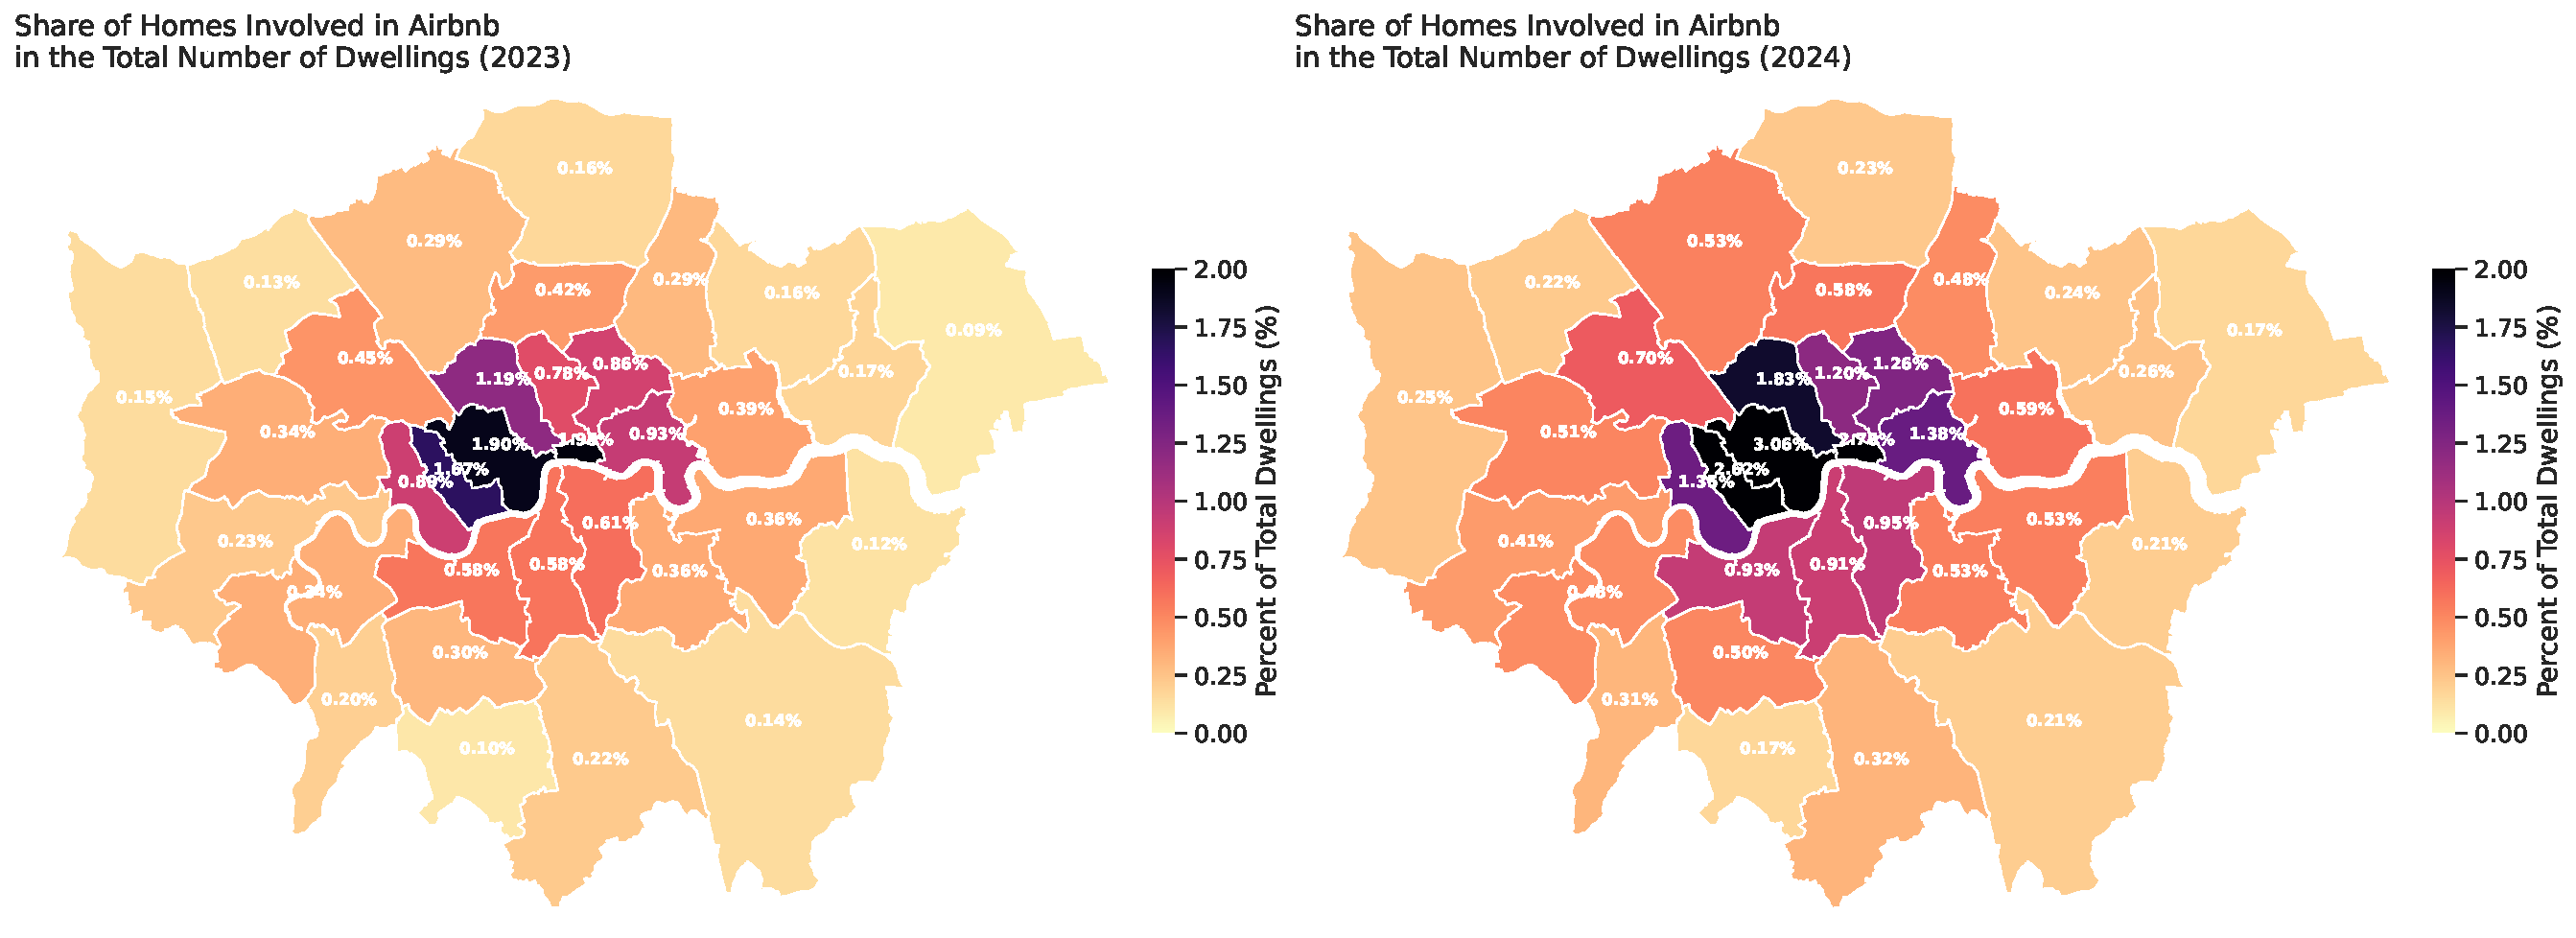
\includegraphics[keepaspectratio]{Group_Work_Template_files/figure-pdf/cell-39-output-1.pdf}}

\subsection{\texorpdfstring{7. Drawing on your previous answers, and
supporting your response with evidence (\emph{e.g.} figures, maps,
EDA/ESDA, and simple statistical analysis/models drawing on experience
from, e.g., CASA0007), how \emph{could} the InsideAirbnb data set be
used to inform the regulation of Short-Term Lets (STL) in
London?}{7. Drawing on your previous answers, and supporting your response with evidence (e.g. figures, maps, EDA/ESDA, and simple statistical analysis/models drawing on experience from, e.g., CASA0007), how could the InsideAirbnb data set be used to inform the regulation of Short-Term Lets (STL) in London?}}\label{drawing-on-your-previous-answers-and-supporting-your-response-with-evidence-e.g.-figures-maps-edaesda-and-simple-statistical-analysismodels-drawing-on-experience-from-e.g.-casa0007-how-could-the-insideairbnb-data-set-be-used-to-inform-the-regulation-of-short-term-lets-stl-in-london}

\subsubsection{Potential link between STL and housing crisis in
London}\label{potential-link-between-stl-and-housing-crisis-in-london}

Despite a narrowing rent-wage gap, rising living costs force low-income
Londoners to spend up to 77\% of wages on housing. Higher mortgage rates
further exclude many from homeownership, disproportionately impacting
vulnerable populations, leading to poverty, evictions, overcrowding, or
homelessness Bevan (2023). There are many claims that STLs exacerbate
this housing crisis, pushing the demand down to the social and private
rental sector. In February 2024, the UK government announced reforms
requiring planning permission for STLs exceeding 90 nights, and a
mandatory STL registration scheme (GOV.UK, 2024b) that will close the
STL data availability gap, discussed in Q4. Additionally, the furnished
holiday lettings tax regime will be abolished (GOV.UK, 2024a). These
continuous efforts aim to keep homes available for local communities.
Airbnb claims no link between listing growth and rising housing costs,
backed by studies discussed in Q6. A caveat of published studies is
their UK-wide statistics for some parameters, which may not reflect
London's heated STL market. With Airbnb comprising 47\% of European
platform STL supply and 30\% across all types, STL impacts on housing
may be more significant Hat. \#\#\# Our research We base our research on
the independent studies conducted in 2019 and 2020 James Todd (2021).
Our goal is to identify proxies accounting for the impacts of the Airbnb
listings on housing in London. We utilise the methodology outlined in
the articles above. \#\#\# Datasets: * InsideAirbnb - see Q6 for
details. * London Boroughs' administrative boundaries provide a
foundation for decision-makers to conduct further analysis. * LSOA 2021
represent smaller geographies. Issues include potential
misrepresentation of demographics, exclusion of daytime populations, and
being too granular for effective citywide visualisation. * Census 2021
provides the most accurate population data, but results may be skewed
due to limited mobility and migration during the Covid-19 pandemic.

\subsubsection{Results and
interpretation:}\label{results-and-interpretation}

The model explains about 53\% of the variation in rental prices (R²),
offering a solid understanding of the main factors influencing rent
changes.

\pandocbounded{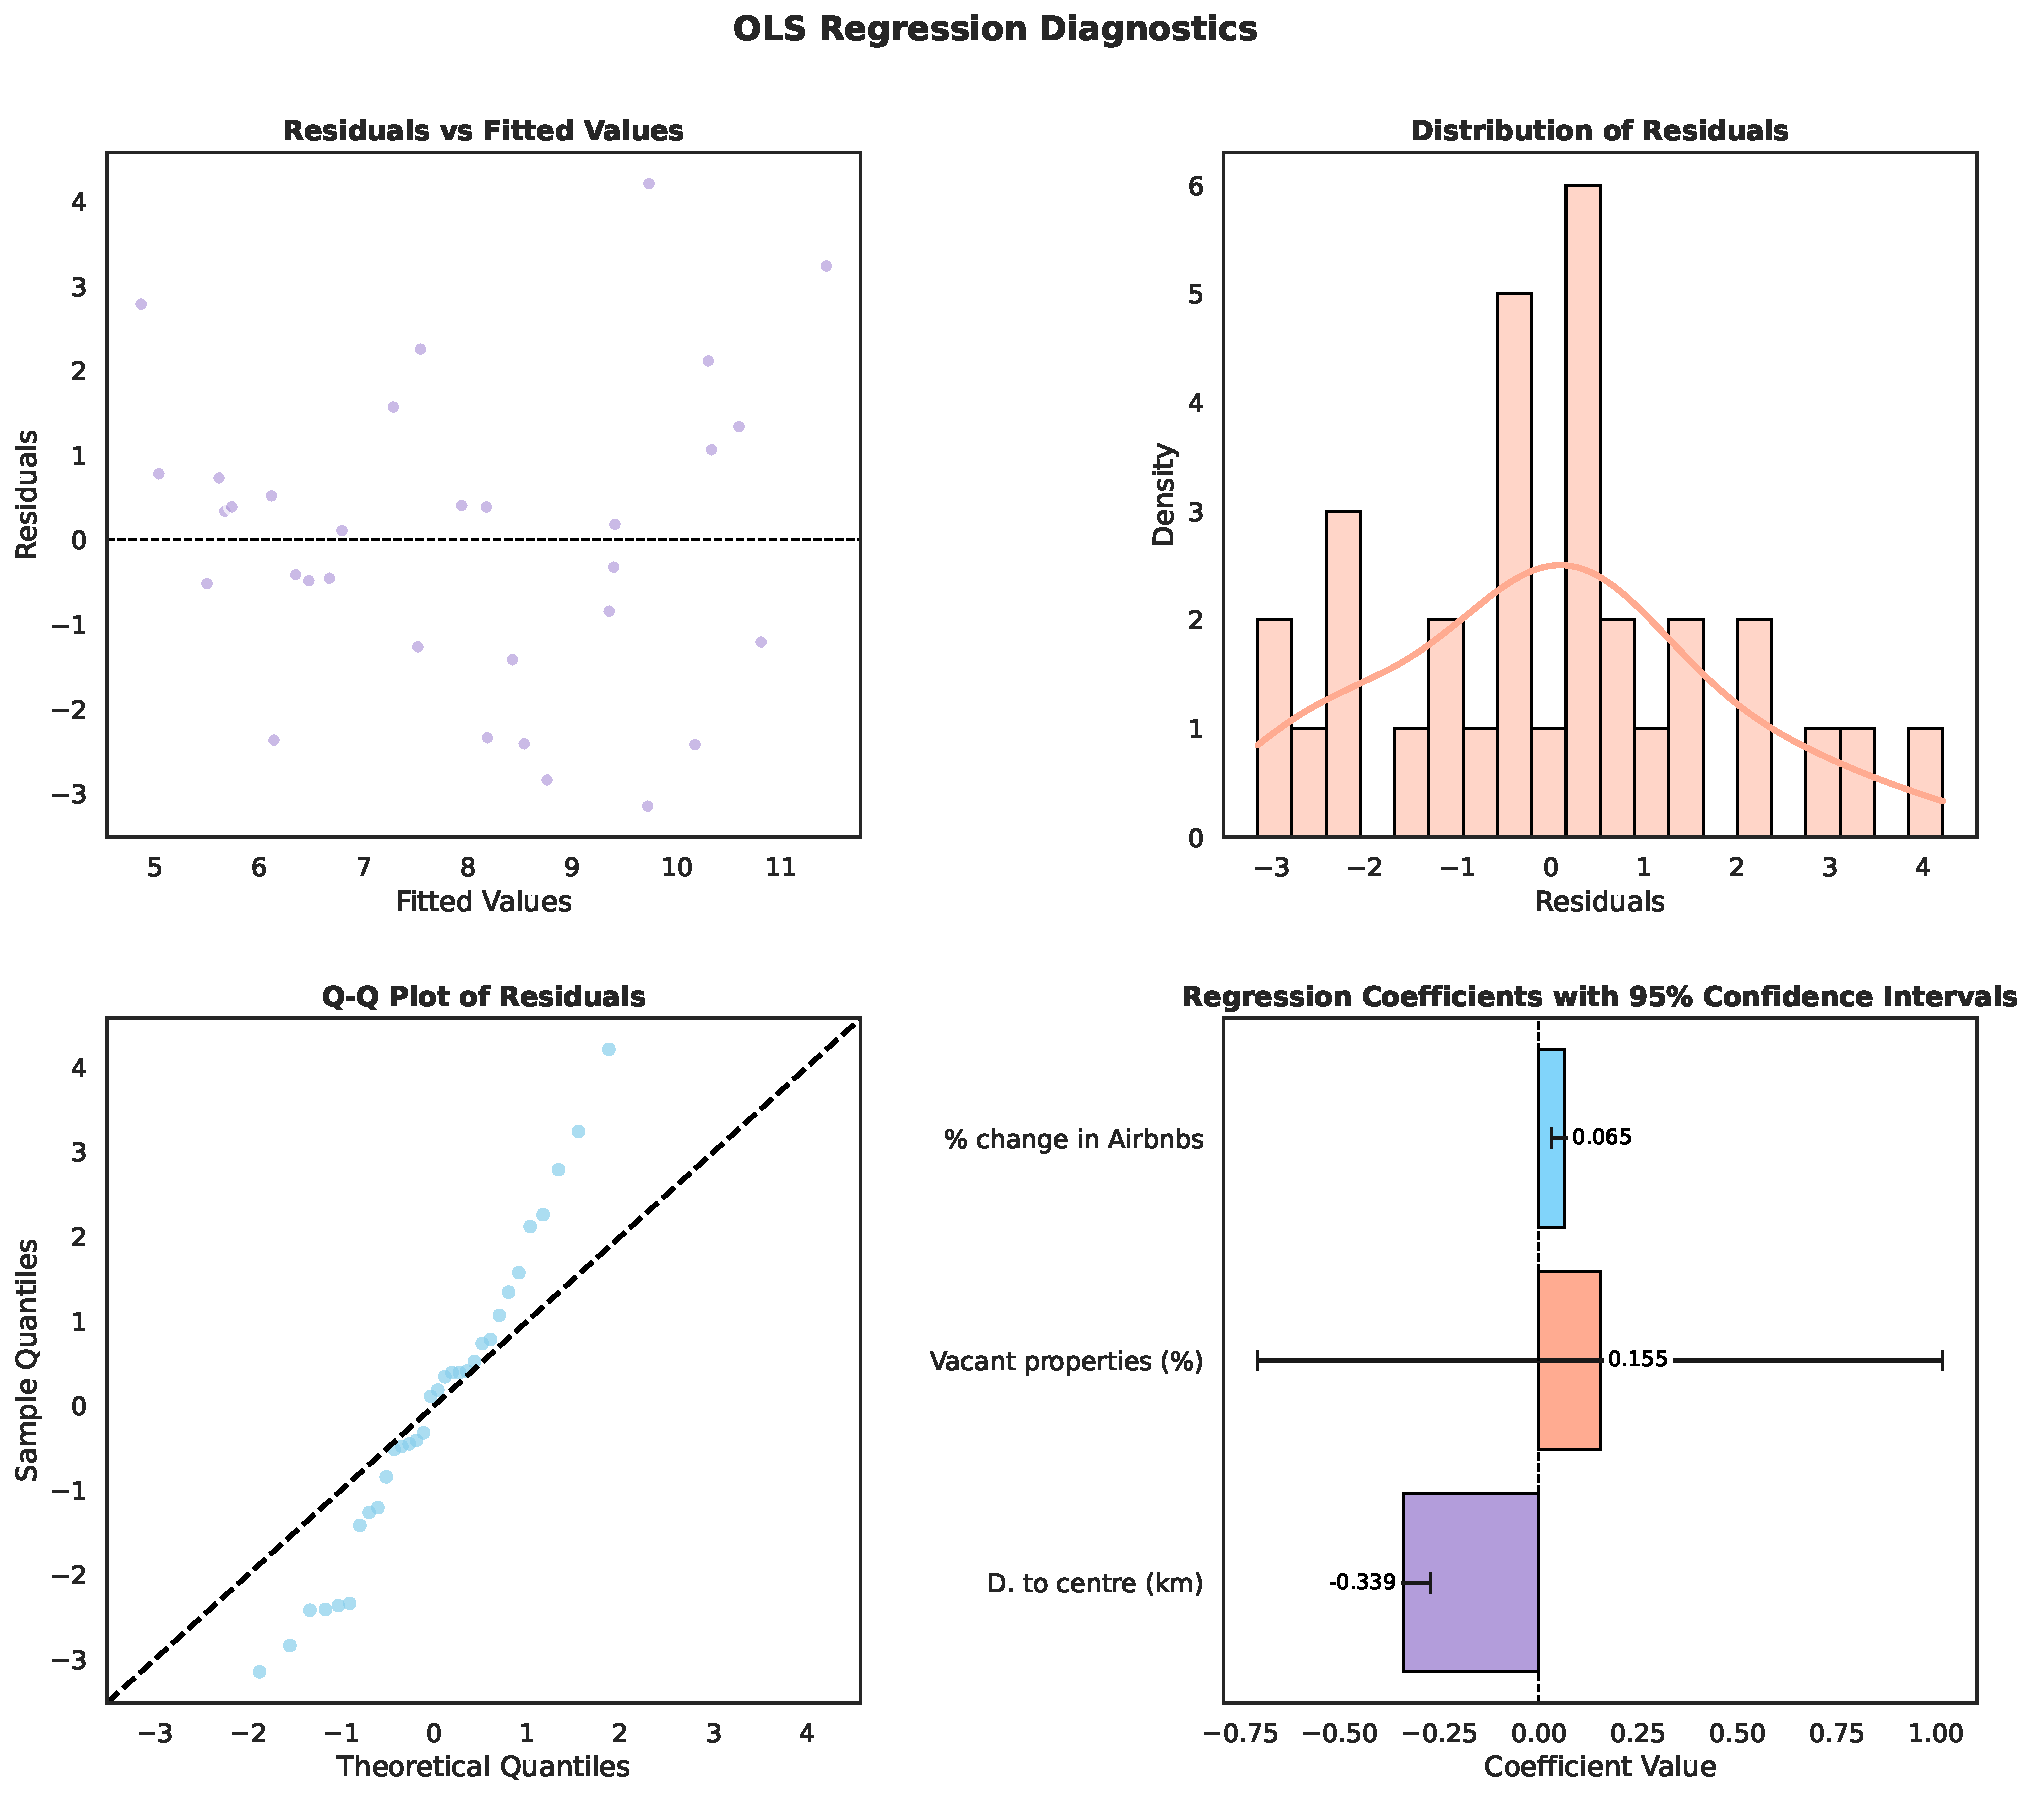
\includegraphics[keepaspectratio]{Group_Work_Template_files/figure-pdf/cell-49-output-1.pdf}}

The model suggests that for every 1\% increase in the number of Airbnb
listings, the change in rental prices grew by 0.065\%. In areas where
Airbnb listings would have doubled, featuring 100\% increase, rents
would have risen by an average of 6.5\%. For tenants, this results in
significant price increases: in central London, where average rents are
around £2,121 per month, a 6.5\% rise would add approximately £138 per
month, or £1,656 per year.

Apart from Airbnb impact, the model results also show that neighborhoods
closer to the centre see an additional 0.34\% increase in rental prices
for every kilometer closer. However, the percentage of vacant dwellings
showed little connection to rent changes.

The story doesn't end with just the numbers. The analysis also revealed
that changes in rental prices are not evenly spread across the city.
Tests on the residuals (errors) displayed uneven patterns in the data,
and further spatial analysis confirmed significant clustering of
residuals.

\pandocbounded{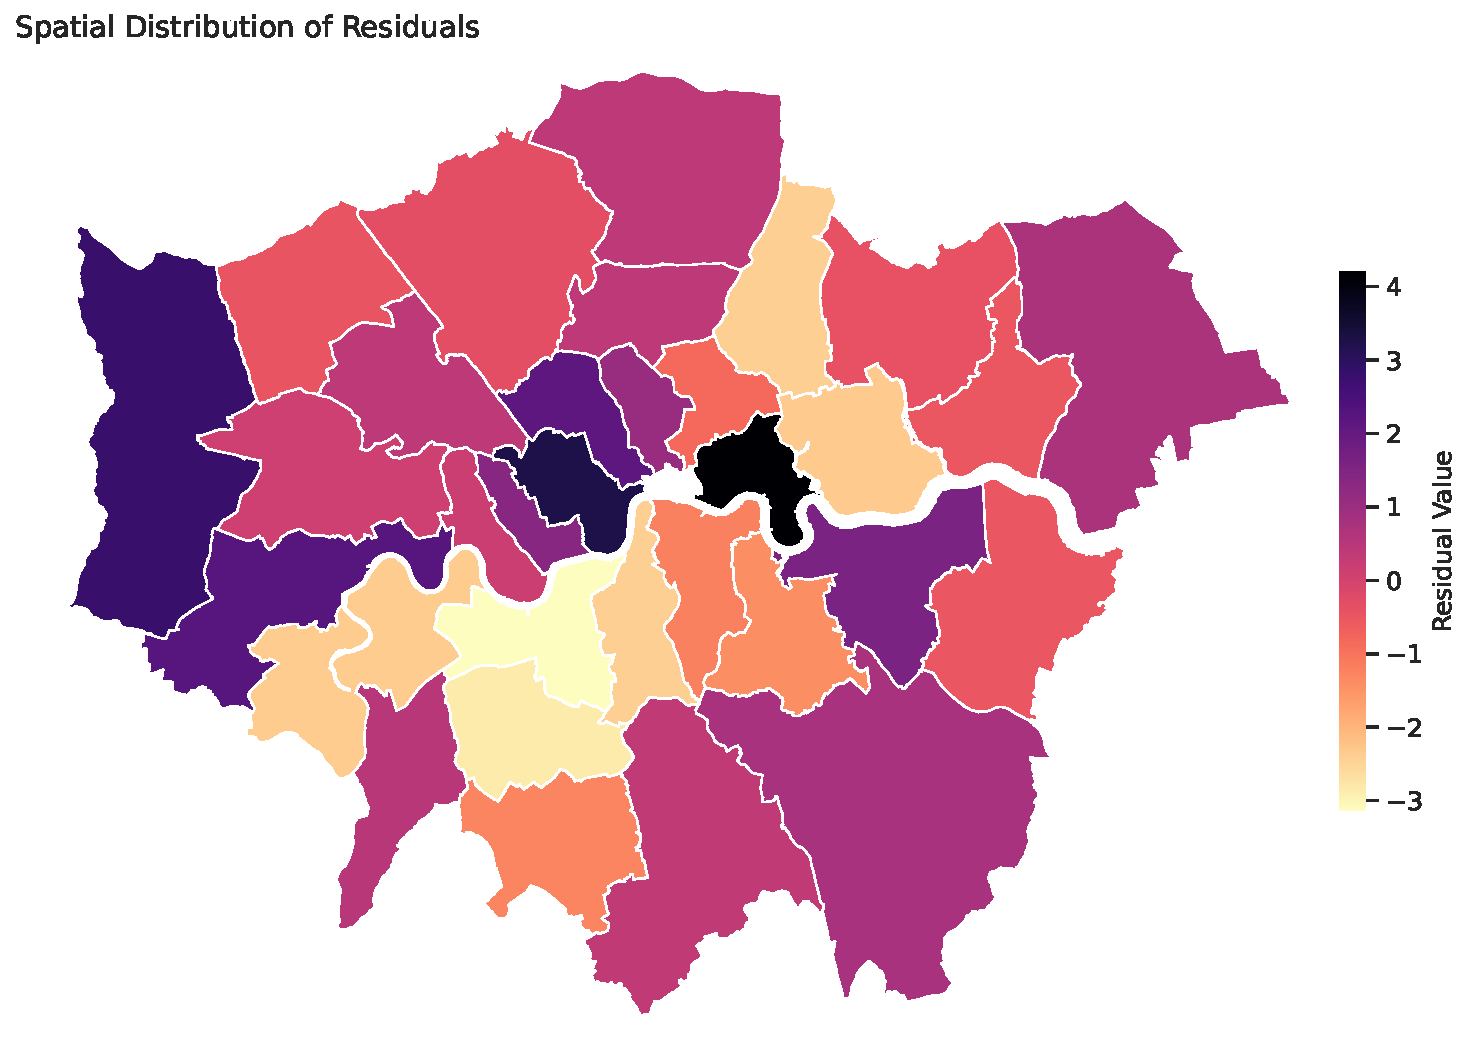
\includegraphics[keepaspectratio]{Group_Work_Template_files/figure-pdf/cell-52-output-1.pdf}}

To build on this analysis, future work could explore how neighborhoods
influence each other by using tools that better capture these spatial
relationships, including Spatial Lag or Spatial Error. Adding more
information, including income levels and housing availability, could
also help explain why rent changes happen in some places but not others.
Additionally, a more robust regression model can be undertaken that
accounts for the uneven spread of residuals.

\subsubsection{Potential analysis
expansion:}\label{potential-analysis-expansion}

Below are the potential additional variables that could be tested in the
future in multiple linear regression: * Social housing waiting times; *
No-fault evictions; * Total new rough sleepers; * Average long-term room
rental prices (e.g.~from Spareroom); * \% or N of Houses of Multiple
Occupancy; * \% or N of flatshare households; * N of Property guardians;
* N of rooms in airbnb compared to n of homes on Airbnb.

\subsubsection{Implications to the regulation of STL in
London:}\label{implications-to-the-regulation-of-stl-in-london}

\textbf{Promote casual STLs} Following the EDA, enforcing the 90-day
rule remains crucial. Multi-listing hosts with large portfolios should
be closely monitored for compliance, as they may duplicate listings to
bypass platform restrictions. A centralized STL registry, as proposed in
February 2024, would enhance transparency, ensure compliance, enable
local councils to monitor STL density and trends, and effectively
distinguish between casual and professional hosts.

\textbf{Encourage private rooms not entire homes} Given the high
concentration of listings, increased pressure on the rental market, and
the 0.34\% rent increase per kilometer closer to the city center, we
propose implementing zoning restrictions in high-demand central boroughs
such as Westminster, Camden, and Kensington \& Chelsea, and in other
areas based on rental market vulnerability, housing supply shortages,
and local socioeconomic conditions. We suggest using spatial models
(e.g., Spatial Lag/Error) to predict areas at risk of STL saturation and
proactively apply regulation. These measures could cap the total number
of listings or limit entire home rentals to encourage private room
listings or overall reduction of the number of listings.

\textbf{Address-based restrictions} The limitations of anonymized data
restrict analysis of property types used for short-term lets. Once the
STL registry is operational, regulations could target specific
addresses, such as affordable housing, social housing, and newly built
properties, to preserve their intended purpose of addressing housing
needs rather than catering to tourists.

\textbf{Redirect STL-generated taxes or fines} There is a potential to
address declining homeownership through redirecting STL taxes or fines
into affordable housing initiatives, supporting vulnerable renters and
first-time buyers. Additionally, introducing an STL tax or levy in these
areas could generate revenue to support affordable housing and community
programs.

\textbf{Long-term rent should be made more profitable} Greater support
is needed to encourage property owners to prioritize long-term rentals
over short-term lets. Currently, STLs are widely promoted as the most
profitable option. Policy solutions could include requiring hosts and
platforms to conduct Social Impact Assessments to evaluate STL impacts
on local housing markets during planning approvals. Additionally,
adjustments to the tax regime for long-term rentals, funded through
redirected STL taxes, could provide further incentives.

\textbf{The landlord should have a choice} Under the new rules,
homeowners will be able to let their primary residence for up to 90
nights annually without planning permission, and dedicated short-term
lets will be automatically reclassified into a new use class. This
approach does not provide landlords sufficient time to assess the
revenue implications, particularly if proposed incentives for long-term
rentals are introduced. The government should reconsider the automatic
reclassification of short-term lets.

\subsection*{References}\label{references}
\addcontentsline{toc}{subsection}{References}

\phantomsection\label{refs}
\begin{CSLReferences}{0}{1}
\bibitem[\citeproctext]{ref-evans2024}
Andy Evans, R.O. (2020) \emph{The impact of short-term lets}. Capital
Economics, p. 32. Available at:
\url{https://www.propertymark.co.uk/static/0165201f-6a7e-46cb-987444e6862ab403/The-impact-of-short-term-lets.pdf}.

\bibitem[\citeproctext]{ref-londonassembly2024}
Assembly, L. (2024) {`How achievable is home ownership for young
londoners?'} Available at:
\url{https://www.london.gov.uk/who-we-are/what-london-assembly-does/london-assembly-press-releases/how-achievable-home-ownership-young-londoners}.

\bibitem[\citeproctext]{ref-bevan2023}
Bevan, D.C. (2023) {`The rise and rise of property guardianship and what
it says about our broken housing system'}. Available at:
\url{https://www.crisis.org.uk/about-us/crisis-media-centre/households-facing-homelessness-from-the-private-rented-sector-reaches-record-levels-in-england-crisis-response/}.

\bibitem[\citeproctext]{ref-finnerty2024}
Catarina Finnerty, R.B. (2023) \emph{Understanding recent rental trends
in london's private rented market}. GLA Housing; Land, p. 18. Available
at:
\url{https://www.london.gov.uk/sites/default/files/2023-06/Housing\%20Research\%20Note\%209\%20-\%20Understanding\%20recent\%20rental\%20trends\%20in\%20London\%27s\%20private\%20rented\%20market.pdf}.

\bibitem[\citeproctext]{ref-crisis2024}
Crisis (2023) {`Households facing homelessness from the private rented
sector reaches record levels in england -- crisis response'}. Available
at:
\url{https://www.crisis.org.uk/about-us/crisis-media-centre/households-facing-homelessness-from-the-private-rented-sector-reaches-record-levels-in-england-crisis-response/}.

\bibitem[\citeproctext]{ref-cromarty2024}
Cromarty, H. (2024) \emph{The growth in short-term lettings in england}.
House of Commons Library, p. 59. Available at:
\url{https://researchbriefings.files.parliament.uk/documents/CBP-8395/CBP-8395.pdf}.

\bibitem[\citeproctext]{ref-GovUK2012}
GOV.UK (2012) {`Live tables on dwelling stock (including vacants)'}.
Available at:
\url{https://www.gov.uk/government/statistical-data-sets/live-tables-on-dwelling-stock-including-vacants}.

\bibitem[\citeproctext]{ref-govuk_abolition2024}
GOV.UK (2024a) {`Abolition of the furnished holiday lettings tax
regime'}. Available at:
\url{https://www.gov.uk/government/publications/furnished-holiday-lettings-tax-regime-abolition/abolition-of-the-furnished-holiday-lettings-tax-regime}.

\bibitem[\citeproctext]{ref-govuk2024}
GOV.UK (2024b) {`Short-term lets rules to protect communities and keep
homes available'}. Available at:
\url{https://www.gov.uk/government/news/short-term-lets-rules-to-protect-communities-and-keep-homes-available}.

\bibitem[\citeproctext]{ref-laymyhat}
Hat, L.M. {`OTA comparison: Airbnb, vrbo, booking, tripadvisor -- what
are they and which should you be using?'} Available at:
\url{https://www.laymyhat.com/portfolio/ota-comparison-airbnb-vrbo-booking-tripadvisor-what-are-they-and-which-is-best-for-owners/}.

\bibitem[\citeproctext]{ref-Todd2021}
James Todd, J.C., Anwar Musah (2021) {`Assessing the impacts of airbnb
listings on london house prices'}. Available at:
\url{https://journals.sagepub.com/doi/full/10.1177/23998083211001836}.

\bibitem[\citeproctext]{ref-kellyk2024}
James W Kelly, N.V. (2024) {`Rise in no-fault evictions in london - city
hall'}. Available at:
\url{https://www.bbc.com/news/articles/c51158xplgxo}.

\bibitem[\citeproctext]{ref-scanlon2024}
Kath Scanlon, C.W., Ellie Benton (2024) \emph{Homesharing for renters:
Barriers and opportunities}. LSE London, p. 39. Available at:
\url{https://www.lse.ac.uk/geography-and-environment/research/lse-london/documents/Reports/240326-LSE-London-Airbnb-Report-A4-WEB-FINAL.pdf}.

\bibitem[\citeproctext]{ref-lighthouse2021}
Lighthouse (2021) {`The ultimate OTA comparison guide: AirBnB vs. VRBO
vs. booking.com'}. Available at:
\url{https://www.mylighthouse.com/resources/blog/vacation-rental-distribution-how-airbnb-vrbo-booking-com-otas-compare}.

\bibitem[\citeproctext]{ref-builtassetmanagement2024}
Management, B.A. (2020) {`New data shows 312'}. Available at:
\url{https://builtassetmanagement.co.uk/blog/\#:~:text=According\%20to\%20our\%20tenant\%20data,in\%20the\%20past\%203\%20years.}

\bibitem[\citeproctext]{ref-powerbiReport2024}
{`Net additional dwellings'} (2024). Ministry of Housing, Communities \&
Local Government. Available at:
\url{https://app.powerbi.com/view?r=eyJrIjoiZTE5YWQ3MDYtZmFjMC00N2YwLWIxM2EtYWY2NTk1NjExYjgwIiwidCI6ImJmMzQ2ODEwLTljN2QtNDNkZS1hODcyLTI0YTJlZjM5OTVhOCJ9}.

\bibitem[\citeproctext]{ref-otte2024}
Otte, J. (2023) {`{``This is just ruinous''}: The britons unable to
afford their homes'}. Available at:
\url{https://www.theguardian.com/society/2023/jun/12/this-is-just-ruinous-the-britons-unable-to-afford-their-homes}.

\bibitem[\citeproctext]{ref-ageuk2024}
UK, A. (2024) {`Home truths: Security for older private renters'}.
Available at:
\url{https://www.ageuk.org.uk/our-impact/campaigning/security-for-older-private-renters/}.

\bibitem[\citeproctext]{ref-EY_Airbnb_2024}
Young LLP, E. \& (2024) \emph{Housing and economic impacts in the UK}.
Ernst \& Young LLP, p. 60. Available at:
\url{https://news.airbnb.com/wp-content/uploads/sites/4/2024/09/EY_Airbnb_Housing-and-Economic-Impacts-in-the-UK.pdf}.

\bibitem[\citeproctext]{ref-Shabrina2021}
Zahratu Shabrina, M.B., Elsa Arcaute (2021) {`Airbnb and its potential
impact on the london housing market'}. Available at:
\url{https://journals.sagepub.com/doi/full/10.1177/0042098020970865}.

\end{CSLReferences}




\end{document}
